\documentclass{article}

\usepackage[pdftex]{geometry}	% Use A4 paper margins
\usepackage[english]{babel}
\usepackage{graphicx}
\usepackage{url}
\usepackage{hyperref}
\usepackage{float}
\usepackage{xcolor} % Required for specifying custom colors
\usepackage{fix-cm} % Allows increasing the font size of specific fonts beyond LaTeX default specifications
\usepackage{tikz}
\usepackage{listings}
\usepackage{pgfplots}
\usepackage{float}
\usepackage{todonotes}
\usepackage{rotating}
\usepackage{pgfplotstable}

\setlength{\oddsidemargin}{0mm} % Adjust margins to center the colored title box
\setlength{\evensidemargin}{0mm} % Margins on even pages - only necessary if adding more content to this template

\newcommand{\HRule}[1]{\hfill \rule{0.2\linewidth}{#1}} % Horizontal rule at the bottom of the page, adjust width here
\renewcommand{\familydefault}{\sfdefault}

\graphicspath{{./images/}}

\begin{document}

\begin{titlepage}

  {\Huge ATX PSU Dev Board }\\
  {\Large Assembly Instructions for v0.1} 
  \vspace*{\fill}	
  \begin{center}
  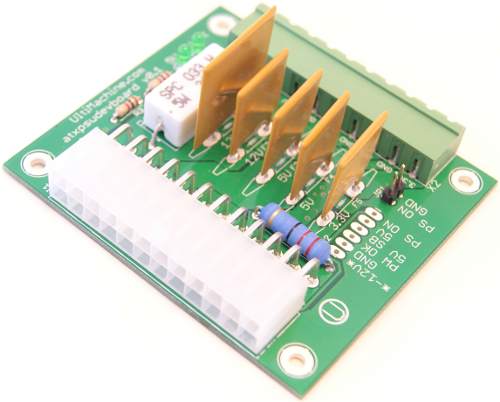
\includegraphics[scale=0.75]{img/ATX_PSU_Dev_PreAssembled2.png}
  \end{center}
  \vspace*{\fill}

  \vfill
  {\centering \large 
  \hfill 
\includegraphics[scale=0.75]{img/um_logo.png} \\
  \hfill \url{http://ultimachine.com/content/atx-psu-dev-board} \\

  \HRule{1pt}} % Horizontal line, thickness changed here
\end{titlepage}

\clearpage % Whitespace to the end of the page

\tableofcontents
\clearpage

\section{Overview}
\subsection{Introduction}


\subsection{What's in the box}
\begin{center}
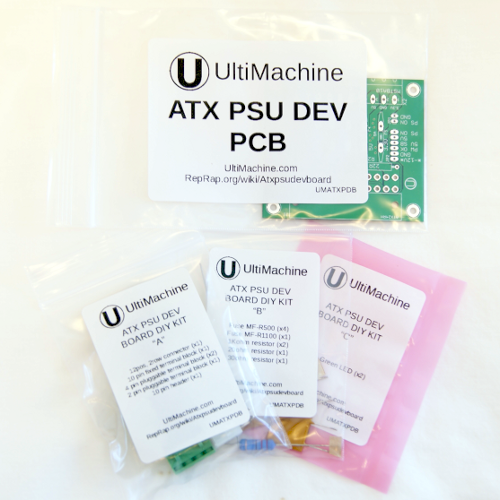
\includegraphics[scale=0.5]{img/ATX_PSU_Dev_DIYkit.png}
\end{center}
\section{Assembly}
\subsection{Preparation}
\subsubsection{Tools}
  The following tools and materials are required to assemble the ATX PSU Dev Board:
    \begin{itemize}
      \item{Soldering Iron}
      \item{Solder}
      \item{Flush/diagonal cutters}
    \end{itemize}
  Additional tools that might be helpful, but not required:
    \begin{itemize}
      \item{Lead bender}
    \end{itemize}

\subsubsection{Soldering}
  If you do not have prior experience soldering, we recommend checking out a few of the following websites for some tutorials. \\
    \url{http://mightyohm.com/files/soldercomic/FullSolderComic_EN.pdf} \\
    \url{http://www.ladyada.net/media/common/soldering.pdf} \\
    \url{http://store.curiousinventor.com/guides/How_to_Solder} \\
    \url{http://www.sparkfun.com/tutorials/106} \\
    \url{http://radiojove.gsfc.nasa.gov/telescope/soldering.htm}

\subsection{Assembly}
  The components of this board will be inserted on the side with the outlines\\

  <Right side, wrong side>
  \\
  Begin by inserting the two 1k$\Omega$ resistors and the LEDs into the board. The LEDs should have the longest lead in the hole facing the resistor. If they are inserted incorrectly they will not work. Resistors are not polarized components, so they can be inserted in orientation. \\

  <Picture of the components in place, inserting long lead.> 
\\
  Next flip over the board and solder the components in. \\

<Soldered the components in> \\

  The fuses will be inserted next. They have a coating that slightly descends down the leads. \\

<Image of the coating>\\

 In order to make a good connection the fuses should slightly hover over the holes. This is so the coating on the leads does not interfere with soldering. You want to bring the fuse above the board. You can do this with RepRap filament or something else, such as a long screw. The orientation of the fuses does not matter. \\

<image of the spaced out fuses> \\   

Next you will want to solder in the remaining resistors. Again, orientation does not matter for resistors.

<Adding resistors to the board. soldered> \\

Now is a good opportunity to check that all connections were soldered well. Ideally the solder should wick up the lead onto the other side of the board. It should also have a nice tapered look. Add some flux and reheat the joint to touch-up the connections if needed. \\

<Examples of good and bad solder joints> \\

Next you will want to add the ATX connector. It has barbs on the housing that should clip onto the circuit board. 

\section{Usage}

\section{Source}

\end{document}
